\section{拐点辅助敏感性及构造}
\label{sec:sup:inflection}
\subsection{相对位置的参数敏感性}
\label{sec:s1:inflection-position}
\begin{proposition}
\label{prop:s1:lambda-sensitivity}
在触发条件及 $S_c<2\bar S<S^*$ 下，固定其余参数，有
\[
\frac{\partial\lambda}{\partial\eta}<0,\qquad
\frac{\partial\lambda}{\partial c_0}>0,\qquad
\frac{\partial\lambda}{\partial\beta}>0.
\]
$\partial\lambda/\partial q_0$ 在允许参数域中可正可负，其驻点满足
\begin{equation}
\frac{\ln[(S^*-\bar S)/\bar S]}{(1-q_0)[\beta+q_0(1-\beta)]}
=-\frac{\ln[\bar S/(S_c-\bar S)]}{S^*-\bar S}
\frac{\partial S^*}{\partial q_0}.
\label{eq:s1:lambda-q0-stationary}
\end{equation}
\end{proposition}
\begin{proof}
记 $A=\ln[(S^*-\bar S)/\bar S]>0$、$B=\ln[\bar S/(S_c-\bar S)]>0$，则
\[
\frac{\partial\lambda}{\partial p}
=\frac{B\,\partial A/\partial p-A\,\partial B/\partial p}{(A+B)^2}.
\]
关于 $\eta$，$\partial A/\partial\eta=(\partial S^*/\partial\eta)/(S^*-\bar S)<0$，且 $\partial B/\partial\eta=0$。
关于 $c_0$，
\[
\frac{\partial A}{\partial c_0}=
\frac{\partial S^*/\partial c_0+S^*/c_0}{S^*-\bar S}>0,
\qquad \frac{\partial B}{\partial c_0}=0.
\]
关于 $\beta$，
\[
\frac{\partial A}{\partial\beta}
=\frac{\partial S^*/\partial\beta+S^*/[\beta(1-\beta)]}{S^*-\bar S}>0,
\qquad
\frac{\partial B}{\partial\beta}
=-\frac1{(1-\beta)[\beta+q_0(1-\beta)]}<0.
\]
这些符号给出前三个结论。最后，
\begin{equation}
\frac{\partial\lambda}{\partial q_0}
=\frac1{(A+B)^2}\left[
\frac{B}{S^*-\bar S}\frac{\partial S^*}{\partial q_0}
+\frac{A}{(1-q_0)[\beta+q_0(1-\beta)]}\right].
\label{eq:lambda-q0-sign}
\end{equation}
令方括号为零得到驻点条件。两项异号本身不足以证明导数能取两种符号；第\ref{app:lambda}节给出两个满足全部条件的参数点，并分别证明其导数为正和负。
\end{proof}

主要符号结果汇总于表\ref{tab:sensitivity}。对于 $q_0$，导数可以变号表示不存在覆盖整个允许参数域的统一方向，不表示每一条固定其他参数的曲线都非单调。
\subsection{拐点的数值分析}

图~\ref{fig:s1:lambda-sensitivity} 给出 $\lambda$ 随 $\eta/N,c_0,\beta,q_0$ 的变化。
在内部拐点存在的范围内，$\lambda$ 随 $\eta$ 增大而减小，随 $c_0$ 和 $\beta$ 增大而增大，与命题~\ref{prop:s1:lambda-sensitivity} 一致。
固定 $N=763,S_0=762,I_0=1,\gamma=0.3504,c_0=10,\eta/N=0.05$，在 $q_0\in[0,0.39]$ 内得到以下局部极大值位置：
\[
\begin{array}{c|ccc}
\beta & 0.10 & 0.12 & 0.155\\
\hline
q_0^\dagger
&0.0736525&0.1969606&0.3890712
\end{array}
\]
这三个位置两侧的 $\frac{\partial \lambda}{\partial q_0}$ 均由正变负，且极大值位置随 $\beta$ 增大而增大。这是所考察参数范围内的数值结果，不涉及一般参数下驻点的唯一性。


\begin{figure}[htbp]
\centering
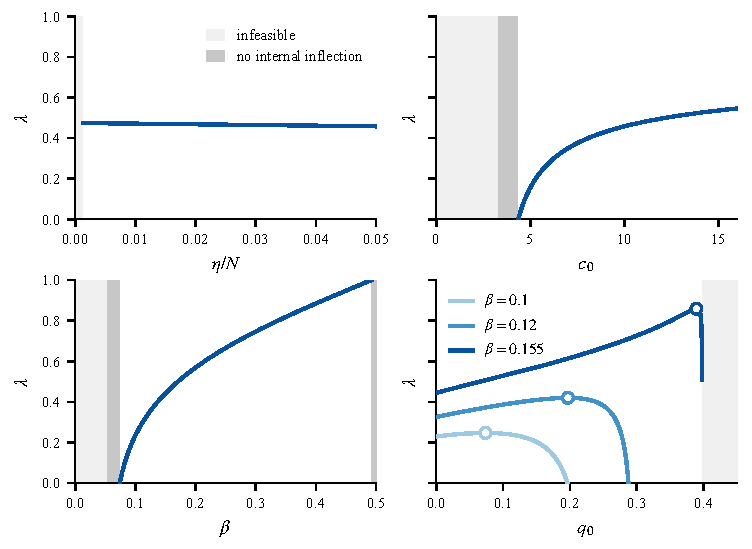
\includegraphics[width=0.8\textwidth]{figures/layout_v5/scenario1_inflection_lambda_sensitivity.pdf}
\caption{拐点相对位置 $\lambda$ 随 $\eta/N,c_0,\beta,q_0$ 的变化。基准取 $N=763,S_0=762,I_0=1,\beta=0.155,\gamma=0.3504,c_0=10,q_0=0.01526,\eta/N=0.05$；$q_0$ 面板另比较 $\beta=0.10,0.12,0.155$。空心圆表示数值局部极大值，浅灰区域表示不满足触发条件，深灰区域表示已触发控制但无内部拐点。$q_0$ 面板的灰色区域对应 $\beta=0.155$。}
\label{fig:s1:lambda-sensitivity}
\end{figure}


改变 $\beta$ 时，两端的拐点边界均可能出现；改变 $c_0$ 时，内部拐点在 $S^*=2\bar S$ 处出现。对于图示的 $q_0$ 和 $\eta/N$ 范围，只要满足控制触发条件，内部拐点就存在。由于 $\qinf$ 仅依赖于 $\beta$，其值在其余三个参数的比较中保持不变。相应的隔离比例时间轨迹见图~\ref{fig:s1:inflection-scan}。


\begin{figure}[htbp]
\centering
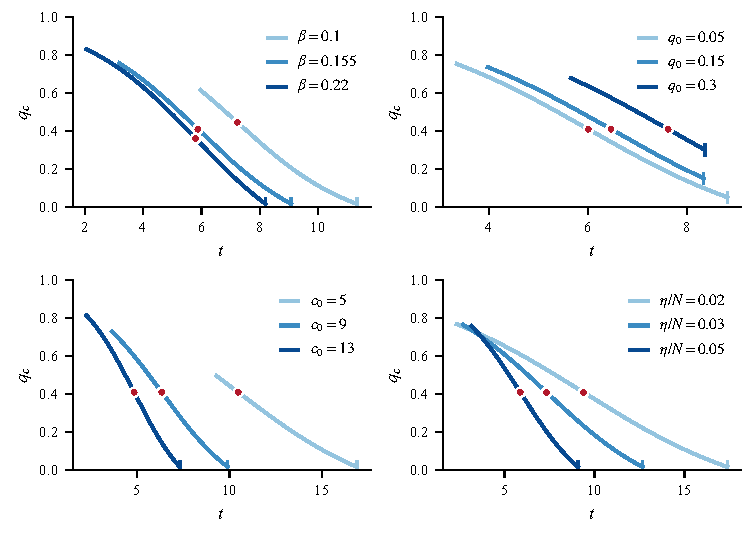
\includegraphics[width=0.8\textwidth]{figures/layout_v5/scenario1_inflection_scan_t.pdf}
\caption{不同 $q_0,\beta,c_0,\eta/N$ 下的隔离比例时间轨迹。其余参数同图\ref{fig:s1:lambda-sensitivity}。圆点为内部拐点，短竖线为控制结束时刻 $t_2$。横轴 $t$ 的单位为天。}
\label{fig:s1:inflection-scan}
\end{figure}


第\ref{app:c0_beta}节 给出了 $(c_0,\beta)$ 平面上的拐点存在范围。固定 $\theta=0.002$、$q_0=0.3230$ 时，西安参数 $(c_0,\beta)=(12.8872,0.1498)$ 位于该范围内。


\FloatBarrier

\subsection{拐点位置关于常规隔离比例的两种变化方向}
\label{app:lambda}
为验证式\eqref{eq:lambda-q0-sign}确实可正可负，取
\[
N=10^6,\quad \beta=\frac16,\quad q_0=\frac1{10},\quad
\gamma=\frac1{10},\quad c_0=\frac{20}{3},\quad I_0=100.
\]
此时 $\beta_2^0/\beta_1^0=3/5,S_c=N/10,\bar S=3N/40$。固定 $S^*=N/5$，对 $r\in\{21/20,2\}$ 分别构造
\[
S_0=rS^*,\qquad
\eta=I_0+\frac{\beta_2^0}{\beta_1^0}(S_0-S^*)+\rho_1\ln(S^*/S_0).
\]
两组参数均有 $S_0+I_0<N$、$I_0<\eta<I_{\max}^{no}$ 和 $S_c<2\bar S<S^*$。余下初始人数可置于不参与社区传播的仓室。在每个构造出的参数点求偏导时，固定该点的 $S_0,\eta$；以上关系仅用于构造参数点，不作为求导时的额外约束。

代入式\eqref{eq:lambda-q0-sign}，得到
\begin{equation}
\frac{\partial\lambda}{\partial q_0}
=\frac{40}{9(\ln5)^2}
\left[\ln\frac53-\ln3\left(\frac{16}{5}(r-1)-\frac65\ln r\right)\right].
\end{equation}
当 $r=21/20$ 时，圆括号中的量在 $0$ 与 $4/25$ 之间。结合 $\ln(5/3)>2/5$、$\ln3<2$，方括号大于 $2/25>0$。当 $r=2$ 时，圆括号中的量大于 $2$；由 $\ln3>2/3$、$\ln(5/3)<2/3$，方括号严格为负。这些估计均可由 $(x-1)/x<\ln x<x-1$（$x>1$）得到，故两种偏导数符号均在允许参数域中实现。

